
%\newpage
\section{Perceptron}\label{sec:perceptron}


\subsection*{Biological vs Artificial Neurons}

A human brain contains billions of neurons, which -- as shown in Figure~\ref{fig:bioneuron} -- are inter-connected nerve cells that are involved in processing and transmitting chemical and electrical signals. Neurons use 
dendrites as branches to receive information from other neurons. The received information is processed by 
the cell body or Soma. A neuron sends information to other neurons through a cable -- called axon -- and the synapse which connects an axon with other neurons' dendrites. 

\begin{figure}[!htbp]
    \centering
    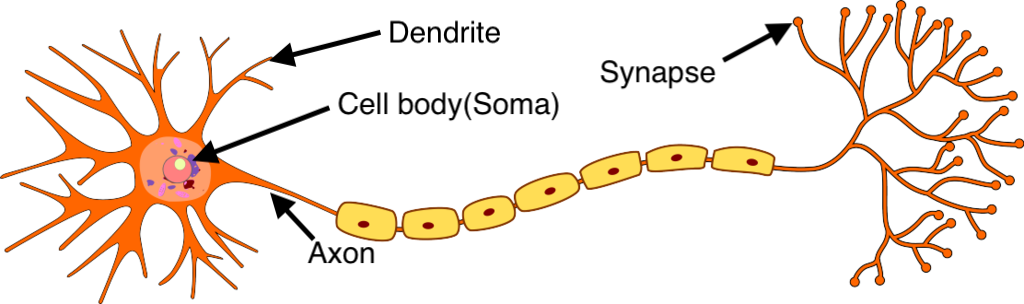
\includegraphics[width=0.7\textwidth]{images/deepLearning/Perceptron/biologicalNeuron.png}
    \caption{Biological Neuron (from Wikipedia)}
    \label{fig:bioneuron}
\end{figure}

In 1943, Warren McCullock and Walter Pitts published a simplified brain cell,  called McCullock-Pitts (MCP) neuron. As shown in Figure~\ref{fig:artneuron}, an artificial neuron represents a nerve cell as a simple logic gate with binary outputs. It takes inputs, weighs them separately, sums them up, and passes this sum through a nonlinear function to produce output. 

\begin{figure}[!htbp]
    \centering
    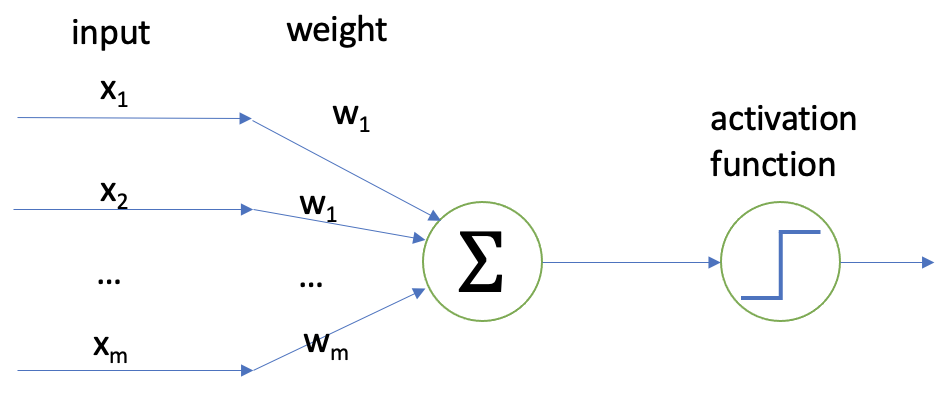
\includegraphics[width=0.6\textwidth]{images/deepLearning/Perceptron/artificialNeuron2.png}
    \caption{Artificial Neuron}
    \label{fig:artneuron}
\end{figure}

Table~\ref{tab:bioartneurons} is a brief conceptual mapping between biological and artificial neurons. 

\begin{table}[!htbp]
    \centering
    \begin{tabular}{|l|l|}
    \hline
       Biological Neuron  &  Artificial Neuron \\
       \hline
        dentrites & input \\
        cell body (soma) & node \\
        axon & output \\
        synapse & weights \\ 
        \hline
    \end{tabular}
    \caption{Mapping of Concepts between Biological and Artificial Neurons}
    \label{tab:bioartneurons}
\end{table}

\subsection*{Learning Algorithm of Perceptron}

A perceptron is an artificial neuron that does certain computations (such as detect features or execute business intelligence) on the input data. 
Perceptron was introduced by Frank Rosenblatt in 1957, when he proposed a perceptron learning rule based on the original MCP neuron. In July 1958, an IBM 704 – a 5-ton computer with the size of a room – was fed a series of punch cards. After 50 trials, the computer taught itself to distinguish cards marked on the left from cards marked on the right \cite{cornell2019}. It was a demonstration of the ``perceptron'', and was ``the first machine which is capable of having an original idea,'' according to its creator, Frank Rosenblatt. 


A perceptron learning algorithm is a  supervised learning of binary classifiers. The binary classifier  processes an input $\textbf{x}=(x_1,...,x_m)$ as follows: 
\begin{enumerate}
    \item Use one weight $w_i$ per feature $X_i$;  
    \item Multiply weights $w_i$ with the  respective input features $x_i$ of $\textbf{x}$, and add bias $w_0$; 
    \item If the result is greater than a pre-specified threshold, return 1. Otherwise, return 0. 
\end{enumerate}

The weights $w_1,...,w_m$ and bias $w_0$ of the binary classifier need to be learned. Given a set $D$ of training instances, the learning algorithm proceeds as follows: 

\begin{itemize}
    \item Initialize weights randomly,
    \item Take one sample $(\textbf{x}_i,y_i)\in D$ and make a prediction ${\hat y}_i$,  
    \item For erroneous predictions,  update weights with the following rules: 
    \begin{itemize}
        \item If the output is ${\hat y}_i=0$ but the label is $y_i=1$, increase the weights. 
       
        \item If the output is ${\hat y}_i=1$ but the label is $y_i=0$, decrease the weights.
    \end{itemize}
    that is, we let 
     \begin{equation}
            w_i=w_i+\Delta w_i \text{~~~~ such that ~~~~} \Delta w_i = \eta(y_i-{\hat y}_i) \textbf{x}_i
        \end{equation}
    where $\eta \ll 1$ is a constant representing the learning rate.
\end{itemize}

\subsection{Expressivity of Perceptron}\label{sec:perceptronexpressivity}

While simple, perceptron is the foundation of modern deep learning, which  uses a network of perceptrons where there are multiple layers and there are multiple neurons per layer.  
%
Why do we need a multi-layer perceptron (MLP) instead of just a single perceptron? This is a question related to the expressivity of a single perceptron. Actually, as we will show below, a single perceptron can express some useful functions but cannot do well for others. 

\subsection*{Linearly separable function} 

As perceptron is a linear classifier, it is able to work well on all linearly separable datasets, i.e., classify instances that can be separated with a linear function. 

\begin{example}
\begin{table}[!htbp]
    \centering
    \begin{tabular}{|c|c||c|}
    \hline
     $X_1$  &  $X_2$   &  \textbf{y} \\
     \hline
      0     & 0  & 0 \\
      0 & 1 & 0 \\
      1 & 0 & 0 \\
      1 & 1 & 1 \\
      \hline
    \end{tabular}
    \caption{Truth table for logic $\land$ (And)}
    \label{tab:truthtableand}
\end{table}
Table~\ref{tab:truthtableand} presents an example dataset of four instances for the logic operator $\land$. Actually, we generalise the logic operator $\land $ to the following function. 
\begin{equation}
    f_\land(x_1,x_2) = 
    \begin{cases}
    1 & \text{ if } x_1 > 0.5 \text{ and } x_2 > 0.5 \\
    0 & \text{otherwise}
    \end{cases}
\end{equation}

In Figure~\ref{fig:logicand}, we use squares to represent 0 and triangles to represent 1. By learning a perceptron, it is possible to get a linear separation function as exhibited in the figure. We use different colors to denote different areas in which the instances should be classified accordingly. In Figure~\ref{fig:logicand}, we also generate a random sample of 100 instances and use the learned perceptron to predict the instances with different colors (with an accuracy close to 1.0).  

\begin{figure}[!htbp]
    \centering
    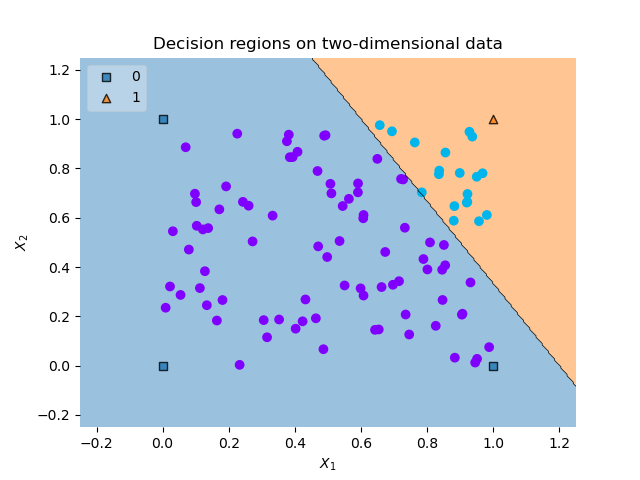
\includegraphics[width=0.7\textwidth]{images/deepLearning/Perceptron/logicand.png}
    \caption{Visualisation of a perceptron learned from the data instances in Table~\ref{tab:truthtableand}}
    \label{fig:logicand}
\end{figure}
\end{example}

\begin{example}
The other example is as shown in  Table~\ref{tab:truthtableor}, presenting  an example dataset of four instances for the logic operator $\lor$. Actually, we generalise the logic operator $\lor $ to the following function. 
\begin{equation}
    f_\lor(x_1,x_2) = 
    \begin{cases}
    1 & \text{ if } x_1 > 0.5 \text{ or } x_2 > 0.5 \\
    0 & \text{otherwise}
    \end{cases}
\end{equation}

\begin{table}[!htbp]
    \centering
    \begin{tabular}{|c|c||c|}
    \hline
     $X_1$  &  $X_2$   &  \textbf{y} \\
     \hline
      0     & 0  & 0 \\
      0 & 1 & 1 \\
      1 & 0 & 1 \\
      1 & 1 & 1 \\
      \hline
    \end{tabular}
    \caption{Truth table for logic $\lor$ (Or)}
    \label{tab:truthtableor}
\end{table}
Figure~\ref{fig:logicor} presents the visualisation of the learned perceptron. We can see that,  the separating line is different from that of Figure~\ref{fig:logicand}. The separating lines in both figures are able to separate the data very well (with accuracy close to 1.0). 
\begin{figure}[!htbp]
    \centering
    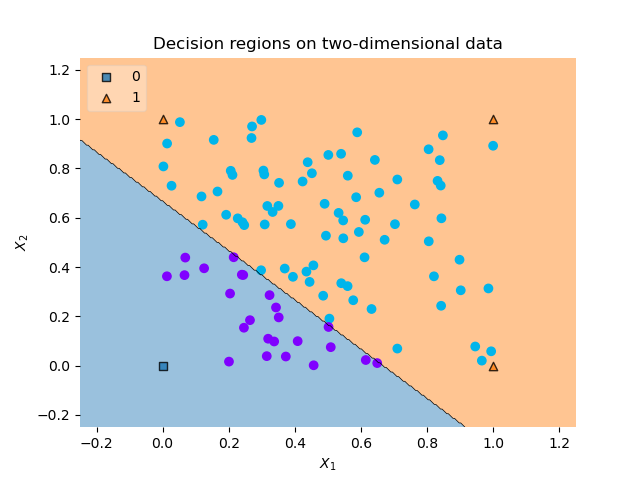
\includegraphics[width=0.7\textwidth]{images/deepLearning/Perceptron/logicor.png}
    \caption{Visualisation of a perceptron learned from the data instances in Table~\ref{tab:truthtableor}}
    \label{fig:logicor}
\end{figure}
\end{example}

The above examples are all based on a 2-dimensional dataset. The learned perceptrons are actually a line on the 2-dimensional space. When the dataset is $d$-dimensional, the perceptron is a $d$-dimensional hyper-plane. 

\subsection*{Linearly inseparable function}

Unfortunately, not all datasets are linearly separable. 

\begin{example}\label{example:xor}
%For example, 
Table~\ref{tab:truthtablexor} is a dataset of four instances, which is generated from the following function:  
\begin{equation}
    f_\oplus(x_1,x_2) = 
    \begin{cases}
    1 & \text{ if } x_1 > 0.5 \text{ and } x_2 < 0.5 \\
    1 & \text{ if } x_1 < 0.5 \text{ and } x_2 > 0.5 \\
    0 & \text{otherwise}
    \end{cases}
\end{equation}
\begin{table}[!htbp]
    \centering
    \begin{tabular}{|c|c||c|}
    \hline
     $X_1$  &  $X_2$   &  \textbf{y} \\
     \hline
      0     & 0  & 0 \\
      0 & 1 & 1 \\
      1 & 0 & 1 \\
      1 & 1 & 0 \\
      \hline
    \end{tabular}
    \caption{Truth table for logic $\oplus$ (XOR)}
    \label{tab:truthtablexor}
\end{table}
While we can still apply perceptron, the learned perceptron cannot reach high accuracy ($\sim$ 0.5 accuracy). 
\end{example}

Therefore, this example shows that the perceptron in itself does not have sufficient expressiveness to work with complex functions. This contributes as the reason why we have to consider multiple layers and more neurons.  

\subsection{Multi-layer Perceptron} 

To deal with the XOR problem, a two-layer perceptron as shown in Figure~\ref{fig:twolayerxor} has been suggested. 

\begin{figure}[!htbp]
    \centering
    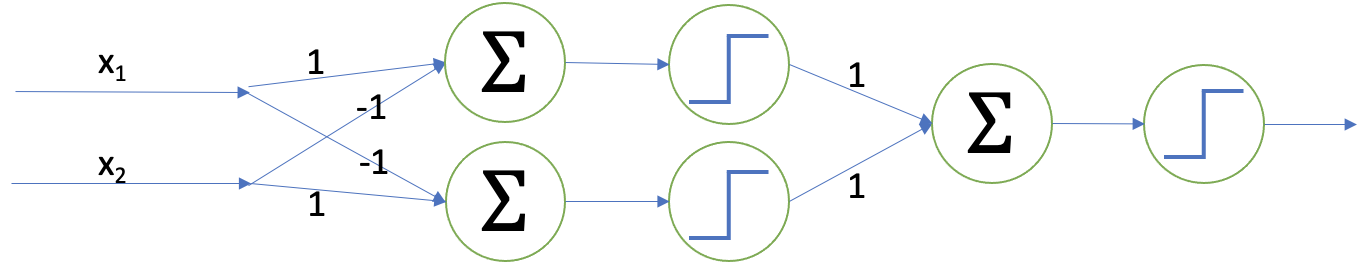
\includegraphics[width=0.7\textwidth]{images/deepLearning/Perceptron/minsky.png}
    \caption{A two-layer perceptron to solve XOR problem}
    \label{fig:twolayerxor}
\end{figure}
where the activation function is $ReLU(x) = \max(0,x)$. 

If written in the matrix form, we have the following expressions for the training data, which shows that the above two-layer perceptron perfectly classifies the training data. 

\begin{equation}
\begin{blockarray}{cc}
\begin{block}{(cc)}
   0 & 0 \\
   0 & 1 \\
   1 & 0 \\
   1 & 1 \\
\end{block}
\end{blockarray}
\times 
\begin{blockarray}{cc}
\begin{block}{(cc)}
   1 & 1 \\
   -1 & 1 \\
\end{block}
\end{blockarray}
=
\begin{blockarray}{cc}
\begin{block}{(cc)}
   0 & 0 \\
   -1 & -1 \\
   1 & -1 \\
   0 & 0 \\
\end{block}
\end{blockarray}
\text{~~ and ~~} ReLU
\begin{blockarray}{cc}
\begin{block}{(cc)}
   0 & 0 \\
   -1 & -1 \\
   1 & -1 \\
   0 & 0 \\
\end{block}
\end{blockarray} = 
\begin{blockarray}{cc}
\begin{block}{(cc)}
   0 & 0 \\
   0 & 1 \\
   1 & 0 \\
   0 & 0 \\
\end{block}
\end{blockarray}
\label{equ:twolayerperceptron}
\end{equation}

\begin{equation}
\begin{blockarray}{cc}
\begin{block}{(cc)}
   0 & 0 \\
   0 & 1 \\
   1 & 0 \\
   0 & 0 \\
\end{block}
\end{blockarray} \times 
\begin{blockarray}{c}
\begin{block}{(c)}
   1  \\
   1  \\
\end{block}
\end{blockarray}
=
\begin{blockarray}{c}
\begin{block}{(c)}
   0  \\
   1  \\
   1  \\
   0  \\
\end{block}
\end{blockarray}
\text{~~ and ~~} 
ReLU
\begin{blockarray}{c}
\begin{block}{(c)}
   0  \\
   1  \\
   1  \\
   0  \\
\end{block}
\end{blockarray} = 
\begin{blockarray}{c}
\begin{block}{(c)}
   0  \\
   1  \\
   1  \\
   0  \\
\end{block}
\end{blockarray}
\label{equ:twolayerperceptron}
\end{equation}

\subsection{Practice}


\subsection*{Train a perceptron}

First of all, we load and prepare datasets. 

\begin{lstlisting}[language=Python]
from sklearn import datasets
dataset = datasets.load_digits()
X = dataset.data
y = dataset.target

observations = len(X)
features = len(dataset.feature_names)
classes = len(dataset.target_names)
print("Number of Observations: " + str(observations))
print("Number of Features: " + str(features))
print("Number of Classes: " + str(classes))

from sklearn.model_selection import train_test_split
X_train, X_test, y_train, y_test = train_test_split(X, y, test_size=0.20)
\end{lstlisting}

Then, we can call \textbf{sklearn}'s library function to train a perceptron model. 

\begin{lstlisting}[language=Python]
from sklearn.linear_model import Perceptron

clf = Perceptron(tol=1e-3, random_state=0)
clf.fit(X_train, y_train)
print("Training accuracy is %s"% clf.score(X_train,y_train))
print("Test accuracy is %s"% clf.score(X_test,y_test))

print("Labels of all instances:\n%s"%y_test)
y_pred = clf.predict(X_test)
print("Predictive outputs of all instances:\n%s"%y_pred)

from sklearn.metrics import classification_report, confusion_matrix
print("Confusion Matrix:\n%s"%confusion_matrix(y_test, y_pred))
print("Classification Report:\n%s"%classification_report(y_test, y_pred))
\end{lstlisting}


\subsection*{Display class regions for Boolean functions}

In the following, we present how to generate the visualisation as in Figure~\ref{fig:logicand} and Figure~\ref{fig:logicor}.
%
First of all, we install a package \textbf{mlxtend}. 

\begin{cmds}
pip3 install mlxtend
\end{cmds}

Then, we need to load the data instances $\textbf{X}=\{(0,0),(0,1),(1,0),(1,1)\}$ and their labels. Note that, in the below code, we use \textbf{logical\_and}. You are able to use others such as \textbf{logical\_or} and \textbf{logical\_xor}. 

\begin{lstlisting}[language=Python]
import numpy as np
# Loading data
X_train = np.array([[0.0,0.0],[0.0,1.0],[1.0,0.0],[1.0,1.0]])
y_train = np.array(np.logical_and(X_train[:, 0] > 0.5, X_train[:, 1] > 0.5), 
             dtype=int)
\end{lstlisting}

Once the data is loaded, we train a Perceptron, with initial parameters $\textbf{w}=(1.5,1.5)$. Note that, this is simply for the experiment, and it can be initialised to other values, or set as default by ignoring the parameter \textbf{coef\_init}. 

\begin{lstlisting}[language=Python]
# Training a classifier
from sklearn.linear_model import Perceptron
clf = Perceptron(tol=1e-3, random_state=0)
clf.fit(X_train, y_train, coef_init=np.array([[1.5],[1.5]]))
\end{lstlisting}

We can print the final learned weights. 

\begin{lstlisting}[language=Python]
print(clf.coef_)
\end{lstlisting}

Finally, we can plot the regions for the classes. 

\begin{lstlisting}[language=Python]
# Plotting decision regions
from mlxtend.plotting import plot_decision_regions
plot_decision_regions(X_train, y_train, clf=clf, legend=2)
\end{lstlisting}

We may also generate a set of random points and plot them. 

\begin{lstlisting}[language=Python]
# Plotting randomly generated points 
import matplotlib
import matplotlib.pyplot as plt
import random

n_sample = 100
X_test = np.array([[random.random() for i in range(2)] for j in range(n_sample)])
y_test = np.array(np.logical_and(X_test[:,0]>0.5,X_test[:,1]>0.5),dtype=int)
y_pred = clf.predict(X_test) 
print(clf.score(X_test,y_test))
colors = matplotlib.cm.rainbow(np.linspace(0, 1, 5))
plt.scatter(X_test[:, 0],X_test[:, 1],color=[colors[i] for i in y_pred])
\end{lstlisting}

\begin{lstlisting}[language=Python]
# Adding axes annotations
import matplotlib.pyplot as plt
plt.xlabel('X_1')
plt.ylabel('X_2')
plt.title('Decision regions on two-dimensional data')
plt.show()
\end{lstlisting}
